\documentclass[dvipsnames]{beamer}
% \mode<presentation>{}
\usepackage[utf8]{inputenc}
\usepackage{amsmath, amssymb, amsfonts, amsthm, mathtools, mathrsfs}
\setbeamertemplate{theorems}[numbered]
\title{Coordinate Hit-and-run}
\author{Amit Rajaraman}
\date[27-11-2021]{27th November 2021}
% \institute{IIT Bombay}
\usetheme{Madrid}
\usepackage{parskip}
\usepackage{tcolorbox}
% \usepackage{tikz-cd}
% \usepackage{commands}
\usepackage{graphicx}
% \usepackage{soul}

% \usepackage{tikz}
% \usetikzlibrary{topaths,calc}
\usepackage{caption}
\usepackage{subcaption}
\usepackage{cancel}
\usepackage{sansmathaccent}
\pdfmapfile{+sansmathaccent.map}

% \tikzset{
%     invisible/.style={opacity=0},
%     visible on/.style={alt={#1{}{invisible}}},
%     alt/.code args={<#1>#2#3}{%
%       \alt<#1>{\pgfkeysalso{#2}}{\pgfkeysalso{#3}}%
%   }
% }

\makeatletter
\newenvironment<>{proofs}[1][\proofname]{%
    \par
    \def\insertproofname{#1\@addpunct{.}}%
    \usebeamertemplate{proof begin}#2}
  {\usebeamertemplate{proof end}}
\makeatother

\newcommand{\R}{\mathbb{R}}
\newcommand{\Rp}{\mathbb{R}^+}
\newcommand{\Rn}{\mathbb{R}^n}
\newcommand{\N}{\mathbb{N}}
\newcommand{\Z}{\mathbb{Z}}
\newcommand{\Q}{\mathbb{Q}}
\newcommand{\vol}{\operatorname{vol}}
\newcommand{\diam}{\operatorname{diam}}
\newcommand{\rad}{\operatorname{rad}}
\newcommand{\norm}[1]{\left\lVert#1\right\rVert}
\newcommand{\grad}{\nabla}
\newcommand{\opnorm}[1]{\norm{#1}_{\text{op}}}
\newcommand{\indic}{\mathbbm{1}}
\renewcommand{\d}[1]{\ensuremath{\operatorname{d}\!{#1}}}
\newcommand{\expec}{\textbf{E}}
\newcommand{\Var}{\operatorname{\textbf{Var}}}
\newcommand{\conv}{\operatorname{Conv}}
\newcommand{\vr}{\operatorname{vr}}
\newcommand{\avg}{\operatorname{avg}}
\newcommand{\med}{\operatorname{med}}
\newcommand{\uvol}{\underline{\vol}}
\newcommand{\ovol}{\overline{\vol}}
\newcommand{\Span}{\operatorname{span}}
\newcommand{\evol}{\widetilde{\vol}}
\newcommand{\Int}{\operatorname{Int}}
\newcommand{\Tr}{\operatorname{Tr}}


% \setbeamercolor{footline}{fg=brown}
% \setbeamerfont{footline}{series=\bfseries}
% \addtobeamertemplate{navigation symbols}{}{%
%     \usebeamerfont{footline}%
%     \usebeamercolor[fg]{footline}%
%     \hspace{1em}%
%     [\insertframenumber/\inserttotalframenumber]
% }

\theoremstyle{definition}
\newtheorem{thm}{Theorem}
\newtheorem{defn}[thm]{Definition}
\newtheorem{prop}[thm]{Proposition}
\newtheorem{cor}[thm]{Corollary}
\newtheorem{caution}[thm]{Caution}
\newtheorem{ques}{Question}
\newtheorem*{alg}{Algorithm}
\newtheorem*{fac}{Fact}
\newtheorem*{ex}{Example}

\DeclareMathOperator{\len}{len}
% \newcommand{\md}[1]{\left\lvert #1 \right\rvert}

\AtBeginSection[]
{
  \begin{frame}
    \frametitle{Table of Contents}
    \tableofcontents[currentsection]
  \end{frame}
}

\begin{document}
\begin{frame}
    \titlepage
\end{frame}

\begin{frame}
    \frametitle{Table of Contents}
    \tableofcontents
\end{frame}

\section{Introduction}
\begin{frame}{The problem}
    Uniformly sampling points from a high-dimensional convex body is a basic problem that relates to problems such as volume computation of convex bodies in high dimensions. \pause \\
    \begin{defn}
        A compact convex body $K \subseteq \Rn$ is said to have a \emph{well-guaranteed membership oracle} if \pause
        \begin{itemize}
            \item it has a \emph{membership oracle}, that is, an oracle that given any $x \in \Rn$ returns whether or not $x \in K$. \pause
            \item we have $R>r>0$ such that $r B_2^n \subseteq K \subseteq R B_2^n$, where $B_2^n$ is the unit ball in the $L_2$ norm in $\Rn$. \pause
        \end{itemize}
    \end{defn}
    Given a well-guaranteed membership oracle for $K$, the problem is to approximately uniformly sample points for $K$.
\end{frame}

\begin{frame}{The problem}
    The B\'{a}r\'{a}ny-Fur\"{e}di Theorem \cite{no-deterministic-algo-barany-furedi} shows that there exists no deterministic polynomial time algorithm to approximate the volume of a convex body. \pause \\
    \begin{ques}
        Input: A convex body $K \subseteq \Rn$ with a well-guaranteed membership oracle.

        Output: A probability distribution on $\Rn$ that is at distance at most $\epsilon$ from the uniform distribution on $K$.
    \end{ques}
\end{frame}

\begin{frame}{The approach in broad strokes}
    The primary method to approximately uniformly sample points is through a \emph{Markov chain}. \pause \\
    We synthesize a Markov chain whose stationary distribution is the uniform distribution on the given body \pause and try to determine how fast we get `close' to this stationary distribution. \pause \\
    The first such random walk\footnote{and consequently, polynomial-time algorithm to approximate the volume of a convex body} was proposed in \cite{dyer-frieze-kannan} by Dyer, Frieze, and Kannan. \pause This random walk was on a grid superimposed on the convex body. \pause
    \begin{center}
    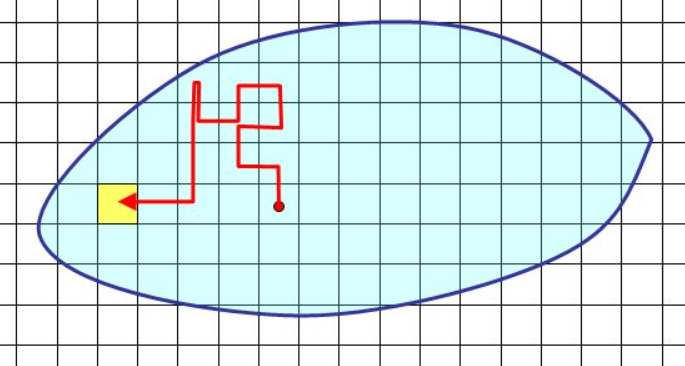
\includegraphics[width = 0.3\linewidth]{dfk-walk.png} 
    \end{center} 
\end{frame}

% \begin{frame}{Na\"{i}ve approach}
%     The simplest way to do this is by \pause trial division. \pause Indeed, we simply divide $n$ by $2, 3, 4$, and so on, and see if the remainder is $0$ in any case. \pause As we know, we only need to divide by numbers up to $\sqrt{n}$. \pause The issue with this algorithm is that it is extremely inefficient, \pause requiring $\Theta(\sqrt{n})$ operations, \pause which is \emph{exponential} in the \emph{bit length} $\log(n)$. \pause For example, if $n$ has $100$-decimal digits, it would take more than $10^{33}$ years to perform $\sqrt{n}$ divisions. \pause

%     Moreover, note that the above algorithm does \emph{more} than what we expected from our algorithm. \pause Namely, it not only tells us that the number is prime but also produces a nontrivial factor in the case that $n$ is composite. 
% \end{frame}

% \begin{frame}{Probabilistic approach}
%     In this talk, we describe a much faster primality testing. \pause This is a polynomial time algorithm. \pause It allows for $100$-decimal digits numbers to be tested in less than a second. \pause Unlike the earlier algorithm, it does \emph{not} give us a prime factor in the case that $n$ is composite. 

%     \pause The catch? \pause This algorithm is \emph{probabilistic}. \pause This means that the algorithm can make a mistake. 

%     \pause \emph{However}, \pause one has control over this probability, and can make it arbitrarily small \pause (but not zero).
% \end{frame}

% \begin{frame}{Some algebraic objects}
%     For the rest of the talk, we shall assume that $n > 1$ is an \emph{odd} integer. \pause
%     Let $n = p_{1}^{e_{1}} \cdots p_{r}^{e_{r}}$ be its prime factorisation. \pause \\
%     By $\mathbb{Z}_{n}$, we shall denote the ring of integers modulo $n$. \pause We have a ring homomorphism
%     \begin{align*} 
%         \theta : \mathbb{Z}_{n} &\to \mathbb{Z}_{p_{1}^{e_1}} \times \cdots \times \mathbb{Z}_{p_{r}^{e_{r}}} \\
%         \uncover<5->{[a]_{n} &\mapsto ([a]_{p_{1}^{e_1}}, \cdots, [a]_{p_{r}^{e_{r}}}).}
%     \end{align*}
%     \pause \pause
%     In fact, the Chinese Remainder Theorems tells us that the above is an isomorphism. \pause This gives us a group isomorphism between the group of invertible elements of the two rings as \pause
%     \begin{equation*} 
%         (\mathbb{Z}_{n})^{\ast} \xrightarrow{\cong} (\mathbb{Z}_{p_{1}^{e_1}})^{\ast} \times \cdots \times (\mathbb{Z}_{p_{r}^{e_{r}}})^{\ast}.
%     \end{equation*}
% \end{frame}

% \begin{frame}{Bird's eye view of probabilistic tests}
%     Several probabilistic primality tests, including the Miller–Rabin test, have the following general structure. \\
%     \pause Define $\mathbb{Z}_{n}^{+}$ to be the set of nonzero elements of $\mathbb{Z}_{n}$. \pause Note that $\md{\mathbb{Z}_{n}^{+}} = n - 1$. \pause Moreover, $\mathbb{Z}_{n}^{+} = \mathbb{Z}_{n}^{\ast}$ iff $n$ is prime. \pause Suppose also that we define a set $L_{n} \subset \mathbb{Z}_{n}^{+}$ such that: \pause
%     \begin{enumerate}[<+->]
%         \item there is an efficient algorithm that on input $n$ and $\alpha \in \mathbb{Z}_{n}^{+}$, determines if $\alpha \in L_{n}$; 
%         \item if $n$ is prime, then $L_{n} = \mathbb{Z}_{n}^{\ast}$; and 
%         \item if $n$ is composite, $\md{L_{n}} \le c(n - 1)$ for some universal constant $c < 1$.
%     \end{enumerate}
%     \pause 
%     To test for primality, we set a ``repetition parameter'' $k$, and choose random elements $\alpha_{1}, \ldots, \alpha_{k} \in \mathbb{Z}_{n}^{+}$. \pause If $\alpha_{i} \in L_{n}$ for all $i \in \{1, \ldots, k\}$, \pause then we output \texttt{true}; \pause otherwise, we output \texttt{false}.
% \end{frame}

% \begin{frame}{Observations}
%     \begin{alg}
%         To test for primality, we set a ``repetition parameter'' $k$, and choose random elements $\alpha_{1}, \ldots, \alpha_{k} \in \mathbb{Z}_{n}^{+}$. If $\alpha_{i} \in L_{n}$ for all $i \in \{1, \ldots, k\}$, then we output \texttt{true}; otherwise, we output \texttt{false}.
%     \end{alg}
%     \pause 
%     \begin{enumerate}   
%         \item The algorithm is efficient since we can check $\alpha \in L_{n}$ efficiently. \pause
%         \item If $n$ is prime, \pause then the algorithm outputs \texttt{true}, \pause and it does so \emph{correctly}. \pause
%         \item If $n$ is composite, \pause then the algorithm \emph{may} output \texttt{true}, \pause with probability at most $c^{k}$.
%     \end{enumerate}

%     \pause In particular, note that there is a \emph{one-sided error}. \pause In fancy language, this is a \emph{Monte Carlo algorithm}.
% \end{frame}

% \section{First attempt}
% \begin{frame}{First attempt}
%     We now try to define a suitable candidate for $L_{n}$. \pause 
%     \begin{defn}
%         \begin{equation*} 
%             L_{n} \vcentcolon= \{\alpha \in \mathbb{Z}_{n}^{+} : {\color{ForestGreen}\alpha^{n - 1} = 1}\}.
%         \end{equation*}
%     \end{defn}
%     \pause 
%     Note that we can test $\alpha \in L_{n}$ efficiently, using a repeated-squaring algorithm.

%     \pause
%     It is easy to see that $L_{n} \subset \mathbb{Z}_{n}^{\ast}$. \pause In fact, $L_{n}$ is the kernel of the $(n - 1)$-power map $\mathbb{Z}_{n}^{\ast} \to \mathbb{Z}_{n}^{\ast}$ given by $x \mapsto x^{n - 1}$.
% \end{frame}

% \begin{frame}{Does it fit the bill?}
%     \begin{thm}
%         If $n$ is prime, then $L_{n} = \mathbb{Z}_{n}^{\ast}$. \pause If $n$ is composite \pause {\only<5->{\color{red}}and $L_{n} \subsetneq \mathbb{Z}_{n}^{\ast}$}, \pause \emph{then} $\md{L_{n}} \le \frac{1}{2}(n - 1)$.
%     \end{thm}
%     \pause \pause
%     \begin{proof}[Proof sketch]
%         The first statement is clear. \pause For the second, one recalls that $L_{n}$ is a subgroup of $Z_{n}^{\ast}$. \pause Thus, $\frac{\md{\mathbb{Z}_{n}^{\ast}}}{\md{L_{n}}}$ is a positive integer. \pause Thus, if the integer is not $1$, it is at least $2$. \pause Combine this with the fact that $\md{Z_{n}^{\ast}} \le n - 1$ to get the result.
%     \end{proof}
%     \pause However, there \emph{are} infinitely many odd composite $n$ for which $L_{n} = \mathbb{Z}_{n}^{\ast}$ \pause and thus, they cannot be ignored.
% \end{frame}

% \begin{frame}{Carmichael numbers}
%     \begin{defn}
%         An odd composite number $n$ such that $L_{n} = \mathbb{Z}_{n}^{\ast}$ is called a \emph{Carmichael number}.
%     \end{defn}
%     \pause
%     \begin{ex}
%         The smallest Carmichael number is $561 = 3 \cdot 11 \cdot 17.$
%     \end{ex}
%     \pause 
%     \begin{thm}
%         $n$ is a Carmichael number iff $n$ is of the following form: \pause
%         \begin{enumerate}[<+->]
%             \item $n = p_{1} \cdots p_{r}$ for distinct primes $p_{i}$,
%             \item {\color{red}$r \ge 3$},
%             \item $(p_{i} - 1) \mid (n - 1)$ for all $i \in \{1, \ldots, r\}$. 
%         \end{enumerate}
%     \end{thm}
%     % \pause The above is not hard to prove, it only requires some basic facts about cyclic groups. However, we skip the proof.
% \end{frame}

% \begin{frame}{Carmichael Numbers characterisation}
%     \begin{proofs} 
%         Let $n = p_{1}^{e_{1}} \cdots p_{r}^{e_{r}}$ be a Carmichael number. \pause From earlier, we have
%         \begin{equation*} 
%             \mathbb{Z}_{n}^{\ast} \cong \mathbb{Z}_{p_{1}^{e_1}}^{\ast} \times \cdots \times \mathbb{Z}_{p_{r}^{e_{r}}}^{\ast}.
%         \end{equation*} \pause
%         Since $n - 1$ annihilates the left group, it annihilates the right group. \pause Thus,
%         \begin{equation*} 
%             p_{i}^{e_{i} - 1}(p_{i} - 1) \mid (n - 1)
%         \end{equation*} 
%         for all $i \in \{1, \ldots, r\}$. \pause In particular, $(p_{i} - 1) \mid (n - 1)$. \pause Moreover, if $e_{i} > 1$ for some $i$, \pause then $p_{i} \mid n - 1$, a contradiction. \pause Thus, $e_{i} = 1$ for all $i$. \pause

%         Now, we must show that $r \ge 3$. \pause For the sake of contradiction, assume that $r = 2$. \pause In this case, we have $n = p_{1} p_{2}$ for some $p_{1} > p_{2}$. \pause We note that
%         \begin{equation*} 
%             n - 1 = p_{1} p_{2} - 1 = (p_{1} - 1) p_{2} + (p_{2} - 1).
%         \end{equation*} \pause
%         The above shows that $p_{1} - 1 \mid p_{2} - 1$, \pause a contradiction since $p_{1} > p_{2}$.
%     \end{proofs}
% \end{frame}
% \begin{frame}{Carmichael Numbers characterisation}
%     \begin{proof}[Proof (Continued)]
%         Conversely, suppose $n$ has the given form. \pause Let $a$ be coprime to $n$ \pause and hence, to each $p_{i}$. \pause Then, by Fermat's Little Theorem, we have $a^{p_{i} - 1} \equiv 1 \mod p_{i}$. \pause Since $n - 1$ is a multiple of $p_{i} - 1$, we get \pause
%         \begin{equation*} 
%             a^{n - 1} \equiv 1 \mod p_{i}
%         \end{equation*}
%         for all $i \in \{1, \ldots, r\}$. \pause By the Chinese Remainder Theorem, we are now done.
%     \end{proof}
% \end{frame}

% \section{The Miller-Rabin test}

% \begin{frame}{A Better Candidate}
%     We now define a new set $L_{n}'$ as follows. \pause
%     \begin{defn}
%         Let $n - 1 = t 2^{h}$ \pause where $t$ is odd, and $h \ge 1$. \pause
%         \begin{align*} 
%             L_{n}' \vcentcolon= \{\alpha \in \mathbb{Z}_{n}^{+} :\ &{\color{ForestGreen}\alpha^{t2^{h}} = 1} \text{ and} \\
%            \uncover<5->{ &{\color{Sepia}\alpha^{t2^{j + 1}} = 1 \Rightarrow \alpha^{t2^{j}} = \pm 1} \text{ for } j = 0, \ldots, h - 1\}. }
%         \end{align*}
%     \end{defn}
%     \pause \pause 
%     The Miller-Rabin test uses this set $L_{n}'$. \pause By definition, it is clear that $L_{n}' \subset L_{n}$, \pause since the {\color{ForestGreen}green condition} is the same from earlier. \pause \\
%     In fact, $L_{n}'$ is precisely the set of those elements of $L_{n}$ which also satisfy the {\color{Sepia}brown condition}.
% \end{frame}

% \begin{frame}{Testing membership}
%     Testing whether a given $\alpha \in \mathbb{Z}_{n}^{+}$ belongs to $L_{n}'$ can be done using the following algorithm: \pause
%     \begin{alg}[Testing membership]
%         \begin{enumerate}[<+->]
%             \itemsep1mm
%             \item $\beta \leftarrow \alpha^{t}$
%             \item if $\beta = 1$ then return \texttt{true}
%             \item for $j \leftarrow 0$ to $h - 1$ do
%             \begin{itemize}[<+->]
%                 \item if $\beta = -1$ then return \texttt{true}
%                 \item if $\beta = 1$ then return \texttt{false}
%                 \item $\beta \leftarrow \beta^{2}$
%             \end{itemize}
%             \item return \texttt{false}
%         \end{enumerate}
%     \end{alg}
%     \pause This algorithm runs in time $O(\mathsf{poly}(\log(n)))$ and thus, satisfies the first criteria.
% \end{frame}

% \begin{frame}{Does it fit the bill?}
%     \begin{thm}
%         If $n$ is prime, then $L_{n}' = \mathbb{Z}_{n}^{\ast}$. \pause If $n$ is composite, then $\md{L_{n}'} \le \frac{1}{4}(n - 1)$.
%     \end{thm}
%     \pause

%     Thus, this set $L_{n}'$ does have the required properties. \pause This choice gives the Miller-Rabin test. \pause 

%     To put it all together, we have the test as:

%     \begin{alg}[Miller-Rabin]
%         \begin{enumerate}[<+->]
%             \itemsep1mm
%             \item input $n$ and $k$
%             \item for $j \leftarrow 1$ to $k$ do 
%             \begin{itemize}[<+->]
%                 \item pick $\alpha \in \mathbb{Z}_{n}^{+}$ randomly
%                 \item if $\alpha \notin L_{n}'$ then return \texttt{false}
%             \end{itemize}
%             \item return \texttt{true}
%         \end{enumerate}
%     \end{alg}
%     \pause 
%     Let us now prove the above theorem.
% \end{frame}
% \begin{frame}{Does it fit the bill? (Yes)}
%     We shall frequently use the following result from group theory: \pause If $G$ has a cyclic group of order $n$, \pause then there are exactly $\gcd(n, m)$ many elements of $G$ satisfying $g^{m} = 1$. \pause
%     \begin{proofs} \pause %Write $n - 1 = t2^{h}$ with $t$ odd. 
%         \textbf{Case 1.} $n$ is prime. 

%         Note that we have $L_{n}' \subset L_{n} = \mathbb{Z}_{n}^{\ast}$. \pause Thus, it suffices to prove that $L_{n} \subset L_{n}'$. \pause But this follows because {\color{Sepia}$x^{2} = 1 \Rightarrow x = \pm 1$} in a field. \\~\\
%         \pause
%         \textbf{Case 2.} $n = p^{e}$ for a prime $p \ge 3$ and $e \ge 2$. \pause

%         Recall that $L_{n}$ is the kernel of the $(n - 1)$-power map. \pause Since $\mathbb{Z}_{n}^{\ast}$ is cyclic, it follows that $\md{L_{n}} = \gcd(\varphi(n), n - 1)$. \pause We can explicitly calculate it to get \pause
%         \begin{flalign*} 
%             \qquad \md{L_{n}'} \le \md{L_{n}} = \only<12>{\gcd(\varphi(n), n - 1)} \only<13>{\gcd(\varphi(p^{e}), p^{e} - 1)} \uncover<14->{\gcd(p^{e - 1}(p - 1), p^{e} - 1) =} \only<15>{p - 1} \uncover<16->{\frac{p^{e} - 1}{p^{e - 1} + \cdots + 1}} \uncover<17->{\le \frac{n - 1}{4}.} &&
%         \end{flalign*}
%     \end{proofs}
% \end{frame}
% \begin{frame}{Does it fit the bill? (Yes)}
%     \begin{proofs}[Proof (continued)]
%         \textbf{Case 3.} $n = p_{1}^{e_{1}} \cdots p_{r}^{e_{r}}$ is the standard prime factorisation of $n$, with $r > 1$. \\~\\\pause
%         %    
%         Let $\theta : \mathbb{Z}_{n} \to \mathbb{Z}_{p_{1}^{e_1}} \times \cdots \times \mathbb{Z}_{p_{r}^{e_{r}}}$ be the ring isomorphism from earlier. \pause \\
%         Write $n - 1 = t2^{h}$ and $\varphi(p_{i}^{e_{i}}) = t_{i}2^{h_{i}}$ in the usual way, \pause and let $g \vcentcolon= \min\{h, h_{1}, \ldots, h_{r}\}$. \pause Note that $g \ge 1$, and that each $\mathbb{Z}_{p_{i}^{e_{i}}}^{\ast}$ is a cyclic group of order $t_{i}2^{h_{i}}$. \pause Let $\alpha \in L_{n}'$. \pause \\~\\
%         %
%         We first show that $\alpha^{t2^{g}} = 1$. \pause By {\color{ForestGreen}definition} of $L_{n}'$, we may assume $g < h$. \pause Now, suppose $\alpha^{t2^{g}} \neq 1$, \pause and let $j$ be the smallest index in $g, \ldots, h - 1$ such that $\alpha^{t2^{j + 1}} = 1$. \pause By {\color{Sepia}definition} of $L_{n}'$, we have $\alpha^{t2^{j}} = -1$. \pause Let $i$ be such that $g = h_{i}$. \pause Writing $\theta(\alpha) = (\alpha_{1}, \ldots, \alpha_{r})$, \pause we have $\alpha_{i}^{t2^{j}} = -1$. \pause Thus, the order of $\alpha_{i}^{t}$ (in $\mathbb{Z}_{p_{i}^{e_{i}}}^{\ast}$) is equal to $2^{j + 1}$. \pause But this is a contradiction since $2^{j + 1}$ does not divide $\md{\mathbb{Z}_{p_{i}^{e_{i}}}^{\ast}} = t_{i}2^{h_{i}}$. \pause \hfill ($\because j \ge g = h_{i}$)
%     \end{proofs}
% \end{frame}

% \begin{frame}{Does it fit the bill? (Yes)}
%     \begin{proofs}[Proof (continued)]
%         For $j = 0, \ldots, h$, define $\rho_{j}$ to be the $(t2^{j})$-power map on $\mathbb{Z}_{n}^{\ast}$. \pause From the previous claim, and the {\color{Sepia}definition} of $L_{n}'$, it follows that $\alpha^{t2^{g - 1}} = \pm 1$ $\forall \alpha \in L_{n}'$. \pause Thus, $L_{n}' \subset \rho_{g - 1}^{-1}(\{\pm 1\})$ \pause and hence, $\md{L_{n}}' \le 2{\color{red}\md{\ker(\rho_{g - 1})}}$. \pause Also,
%         \begin{flalign*} 
%             && \md{\ker(\rho_{j})} = \prod_{i = 1}^{r} \gcd(t_{i}2^{h_{i}}, t2^{j}) && \forall j \in \{0, \ldots, h\}.
%         \end{flalign*}
%         \pause Since $g \le h$ and $g \le h_{i}$ for all $i$, we get \pause
%         \begin{equation*} 
%             {\color{red}2^{r}\md{\ker(\rho_{g - 1})}} = \md{\ker(\rho_{g})} \le \md{\ker(\rho_{h})}.
%         \end{equation*} \pause
%         Combining the {\color{red}red} expressions, we get
%         \begin{equation*} 
%             \md{L_{n}'} \le 2^{-r + 1}\md{\ker(\rho_{h})} = \frac{\md{L_{n}}}{2^{r - 1}}.
%         \end{equation*}
%     \end{proofs}
% \end{frame}

% \begin{frame}{Does it fit the bill? (Yes)}
%     \begin{proof}[Proof (continued)]
%         \begin{equation*} 
%             \md{L_{n}'} \le \frac{\md{L_{n}}}{2^{r - 1}}
%         \end{equation*} \pause
%         If $r \ge 3$, then we are done \pause since $\md{L_{n}} \le \md{\mathbb{Z}_{n}^{\ast}} \le n - 1$, and $2^{r - 1} \ge 4$. \pause 

%         If $r = 2$, then $n$ is not a Carmichael number and thus, \pause 
%         \begin{equation*} 
%             \frac{\md{L_{n}}}{2^{r - 1}} = \frac{\md{L_{n}}}{2} \uncover<6->{\le \frac{1}{4}(n - 1), }
%         \end{equation*} \pause 
%         and we are again done.
%     \end{proof}
% \end{frame}

\bibliographystyle{alpha}
\bibliography{references}

\end{document}